%%%%%%%%%%%%%%%%%%%%%%%%%%%%%%%%%%%%%%%%%%%%%%%%%%%%%%%%%%%%%%%%%%%%%%%%%%%%%%%%%%%%%%%%%%%%%%%%%%%%%%%%%%%%%%%%%%%%%%%%%%%%%%%%%%%%%%%%%%%%%%%%%%%%%%%%%%%%%%%%%%%%%%%%%%%%%%%%%%%%
%%%%%%%%%%%%%%%%%%%%%%%%%%%%%%%%%%%%%%%%%%%%%%%%%%%%%%%%%%%%%%%%%%%%%%%%%%%%%%%%%%%%%%%%%%%%%%%%%%%%%%%%%%%%%%%%%%%%%%%%%%%%%%%%%%%%%%%%%%%%%%%%%%%%%%%%%%%%%%%%%%%%%%%%%%%%%%%%%%%%
\section{Simulated samples}
\label{sec:SimulatedSamples}

For the investigation of the various backgrounds to this search, the analysis relies also on simulated sample.
An extensive introduction to the techniques and tools required for the simulation of SM and beyond SM processes can be found in Section~\ref{FIXME}.

In the following two sections an overview about the used SM (Section~\ref{sec:SMSamples}) and SUSY samples (Section~\ref{sec:SignalSamples}) is given.
All samples are reweighted to match the measured distribution of primary vertices in data.

\subsection{SM Background samples}
\label{sec:SMSamples}
To investigate the sources of background, various simulated SM samples were used.
In order to have the possibility to make use of the $dE/dx$ variables, a special data format of the simulated samples is required (called RECO format).
Unfortunately, not all SM processes were available in this format in which also the information about the energy release in the tracking system is included.
However, as this analysis needs to rely anyways on a data-based background estimation method, because of the limited quality of the $dE/dx$ simulation.
this does not constitute a serious problem, but only limit the possibility of an extensive comparison between data and simulation going beyond shape comparisons.

In Table \ref{tab:SMsamples_RECO} all SM samples are listed which were available in the RECO format and are used in the analysis.
\renewcommand{\arraystretch}{1.5}
\begin{table}[!b]
\centering
\caption{Available and used Standard Model background samples containing $\Delta E/\Delta x$ information.}
\label{tab:SMsamples_RECO}
\makebox[0.99\textwidth]{
\begin{tabular}{lll}
\multicolumn{3}{c}{} \\
\toprule
 Process & Cross section $\left[\pb\right]$ & $\mathcal{O}_{\text{calculation}}$ \\%& Size $\left[\text{TB}\right]$\\
\midrule
 $W$ + jets                                             &  36703.2     &  NNLO \cite{bib:FEWZ} \\%& 70.4 \\
 $t\bar{t}$ + jets                                      &  245.8       &  NNLO \cite{bib:ttbar:Czakon_2013}\\%& 55.9 \\
 Z$\rightarrow\ell\ell$ ($\ell=e,\mu,\tau$)             &  3531.9      &  NNLO \cite{bib:FEWZ} \\%& 5.1  \\
 QCD ($50\gev<\hat{p}_{\text{T}}<1400\gev$)               &  9374794.2    &  LO  \\%% & 44.3\\
\bottomrule
\end{tabular}}
\end{table}  
Due to the immense size of the samples (between 5 and 70\,TB) and in order to match a reasonable storage space a reduction was done by selecting only events which contain at least one leading jet with a minimum transverse momentum of $\pt>60\gev$.

In addition, further simulated samples not containing the energy information are used.
These are needed to study the backgound inclusively in the variable \ias.
They are listed in Table~\ref{tab:SMsamples_AOD}.
\renewcommand{\arraystretch}{1.5}
\begin{table}[!t]
\centering
\caption{Used Standard Model background samples without $\Delta E/\Delta x$ information.}
\label{tab:SMsamples_AOD}
\makebox[0.99\textwidth]{
\begin{tabular}{lll}
\multicolumn{3}{c}{} \\
\toprule
 Process & Cross section $\left[\pb\right]$ & $\mathcal{O}_{\text{calculation}}$ \\%& Size $\left[\text{TB}\right]$\\
\midrule
 $W$ + jets                                                &  36703.2    &  NNLO \cite{bib:FEWZ} \\%& 70.4 \\
 Z$\rightarrow\ell\ell$ ($\ell=e,\mu,\tau$) + 1,2,3,4 jets &  3531.9     &  NNLO \cite{bib:FEWZ} \\%& 5.1  \\
\bottomrule
\end{tabular}}
\end{table}  

%\begin{itemize}
%\item Main Background are ... ???
%\item Most important sample was included: Wjets
%\item ZoNuNu Backgrund not availbale plays also a role (see DT paper!)
%\item Table of SM samples with cross sections
%\end{itemize}

\subsection{Signal samples}
\label{sec:SignalSamples}
For the investigation of a possible signal, events containing either chargino pair production $q\bar{q} \rightarrow \chipm \chimp$ or chargino neutralino production $q\bar{q} \rightarrow \chipm \chiO$ are simulated. 
The simulation is done with the matrix-element event generator \madgraph \cite{bib:Madgraph_2014}
The parton showering and hadronization processes are then simulated with Pythia 6 \cite{bib:Pyhtia6_2006}.
A last step is needed to simulate the interations of the generated particles with the detector material, which is done with \geant \cite{bib:Geant4_2003,bib:Geant4_2006}.

Furthermore, a speacial treatment for long-lived particles is required.
In order to get the right detector simulation of the energy loss of the long-lived particles which decay after the beam pipe, the lifetime of the chargino cannot be set in the matrix-element generator but needs to be specified within \geant.
This also means, that the decay products are only existing in the detector simulation, but are not accessible as particles in the event generators.


To narrow down the required computing sources, the simulation was only done for a few lifetimes (1\cm, 5\cm, 10\cm, 50\cm, 100\cm, 1\,000\cm and 10\,000\cm).
To get still a tight scan over the lifetime space, other lifetimes were generated using lifetime reweighting.
This can be done by determining for every event a weight which is depending on the individual proper lifetime of the chargino (in case of chargino pair production it depends on the individual lifetime of the two charginos).
The event weight is given by
\begin{equation*}
w = \prod_{i=1}^n \frac{\tau^{\text{gen}}}{\tau^{\text{target}}}\cdot  \exp \left[ t_i \cdot \left( \frac{1}{\tau^{\text{target}}} - \frac{1}{\tau^{\text{gen}}} \right) \right] ,
\end{equation*}
where $n$ is the  number of charginos in the event, $\tau^{\text{gen}}$ is the generated mean lifetime in the particle's rest frame and $t_i$ is the individual proper lifetime of the chargino. 
The resulting mean lifetime is then given by $\tau^{\text{target}}$. A derivation of this formula can be found in Appendix~\ref{blabla}.
With the reweighting procedure a tight covering of the lifetime space could be achieved with lifetimes of \ctau = $a\cdot10^{n}$ for $n$=0,1,2,3,4 and $a$=$\left[1,9\right]$.
Figure~\ref{fig:LifetimeReweighting} shows the exponential distribution of the individual proper lifetime of the charginos after reweighting a simulated sample with $c\tau^{\text{gen}}=50\cm$ to a lifetime of $c\tau^{\text{target}}=10\cm$.
Fitting the exponential spectrum should result in the correct mean proper lifetime as parameter of the fit.
It can be seen, that the reweighting procedure can reproduce the targeted lifetime of 10\cm.
\begin{figure}[!t]
  \centering 
  \begin{tabular}{c}
    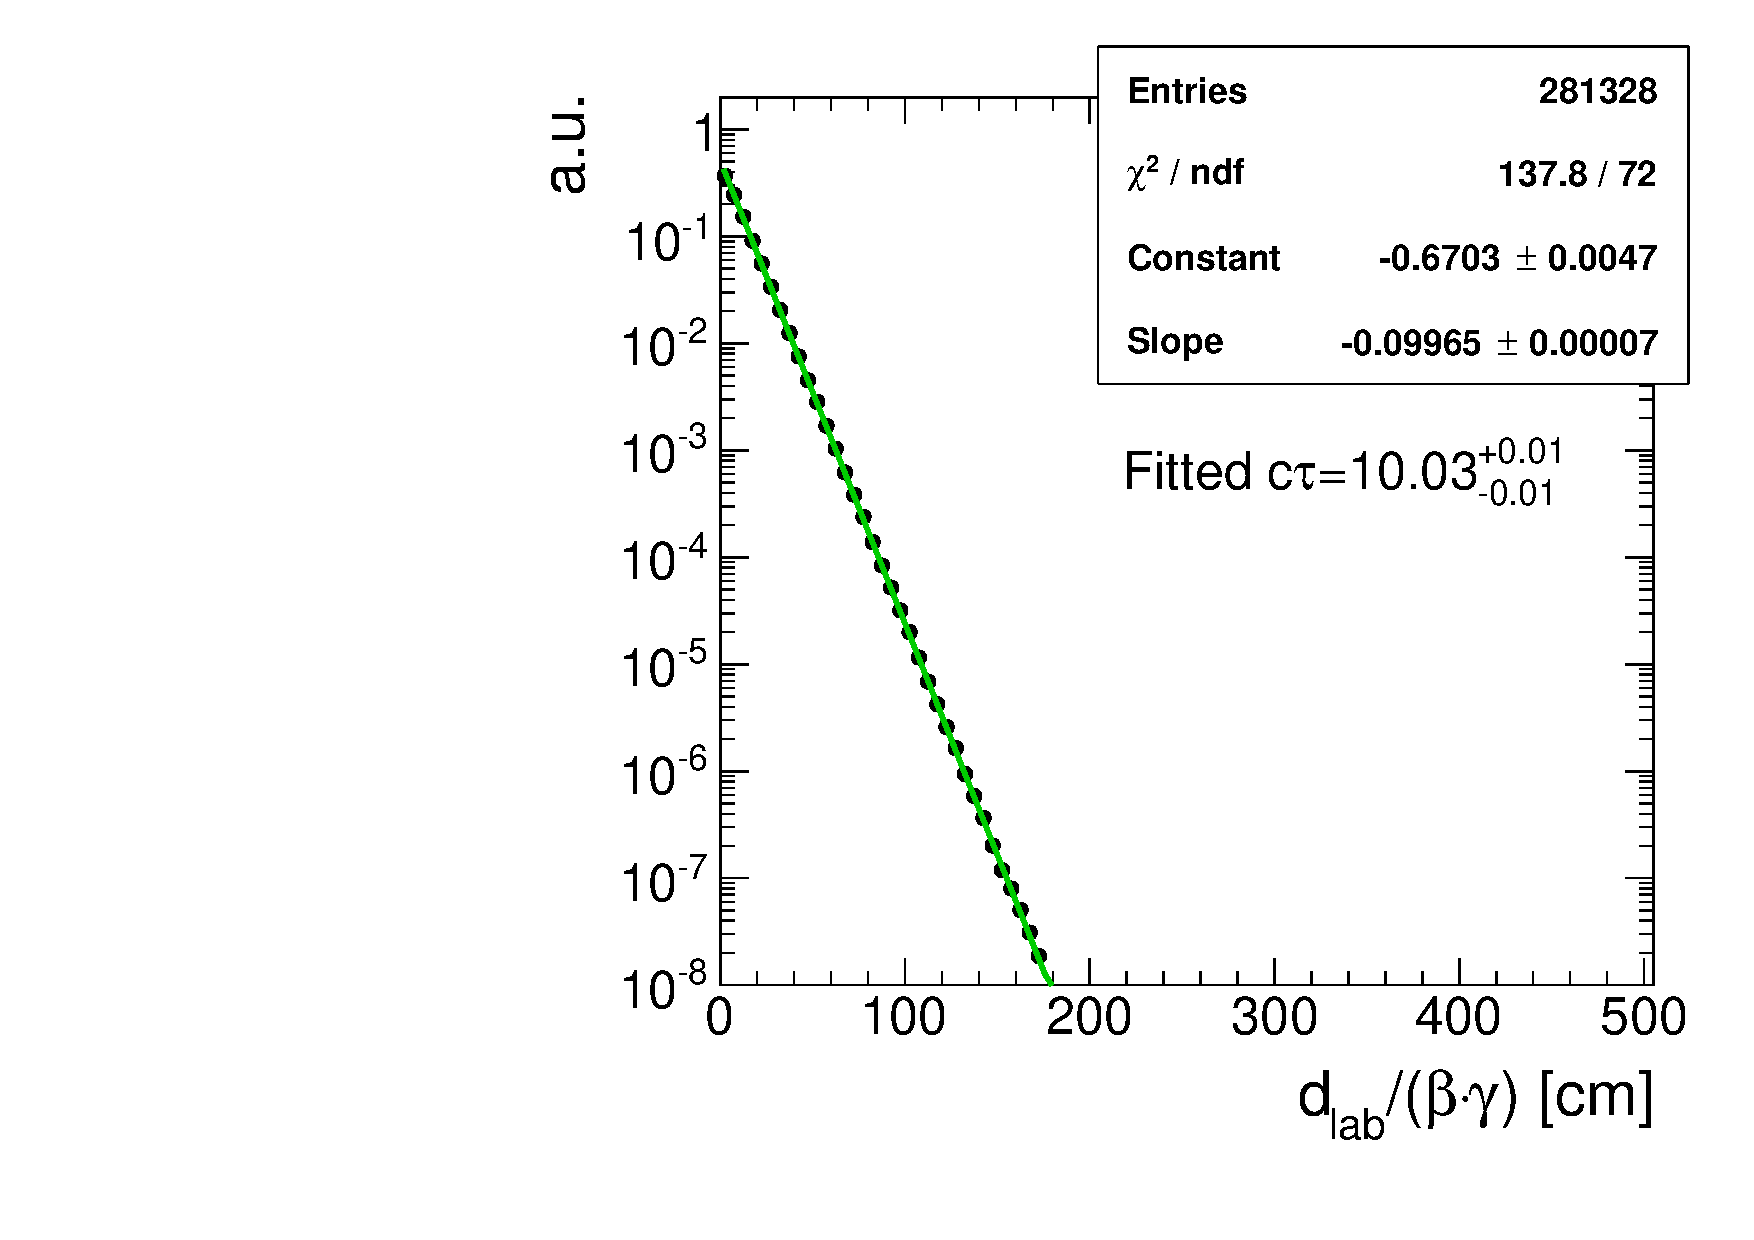
\includegraphics[width=0.49\textwidth]{figures/analysis/10cm.pdf}
  \end{tabular}
  \caption{Normalized distribution of the proper lifetime $d_{\text{lab}}/\left(\beta\gamma \right)$ of all charginos contained in a signal sample with a generated lifetime of $c\tau^{\text{gen}}=50\cm$ reweighted to a lifetime of $c\tau^{\text{target}}=10\cm$.}
  \label{fig:LifetimeReweighting}
\end{figure}


All samples were generated for different chargino masses always almost mass-degenerate to the lightest neutralino.
The mass gap between chargino and neutralino was set to 5\gev.
However, as this analysis does not make use of the other decay products and the lifetime is set in \geant, the mass gap does not play any role.
Six different masses from 100\gev to 600\gev are simulated.
This leads then to a total number of 42 signal samples.
In Table~\ref{tab:SignalCrossSections} the NLO-NLL\footnote{NLO: next-to-leading order, NLL: next-to-leading logarithmic accuracy} cross sections at $\sqrt{s}=8\tev$ for $\chipm\chimp$ and $\chipm\chiO$ production 
with wino-like charginos and degeneracy between $m_{\chipm}$ and $m_{\chiO}$ are listed \cite{bib:SignalCrossSection_2012,bib:SignalCrossSection_2013}.
The cross section does not dependent on the lifetime of the chargino.
\renewcommand{\arraystretch}{1.5}
\begin{table}[!h]
\centering
\caption{Produced signal simulated samples with corresponding cross sections}
\label{tab:SignalCrossSections}
\makebox[0.99\textwidth]{
\begin{tabular}{lll}
\multicolumn{3}{c}{} \\
\toprule
 $m_{\chipm}\left[\gev\right]$ & $\sigma_{\chipm\chimp}\left[\pb\right]$  & $\sigma_{\chiO\chimp}\left[\pb\right]$ \\
\midrule
 100     &  5.8234     &  11.5132 \\
 200     &  0.37924    &  0.77661 \\
 300     &  0.06751    &  0.14176 \\
 400     &  0.01751    &  0.03758 \\
 500     &  0.00553    &  0.01205 \\
 600     &  0.00196    &  0.00431 \\
\bottomrule
\end{tabular}}
\end{table}  
%%%%%%%%%%%%%%%%%%%%%%%%%%%%%%%%%%%%%%%%%%%%%%%%%%%%%%%%%%%%%%%%%%%%%%%%%%%%%%%%%%%%%%%%%%%%%%%%%%%%%%%%%%%%%%%%%%%%%%%%%%%%%%%%%%%%%%%%%%%%%%%%%%%%%%%%%%%%%%%%%%%%%%%%%%%%%%%%%%%%
%%%%%%%%%%%%%%%%%%%%%%%%%%%%%%%%%%%%%%%%%%%%%%%%%%%%%%%%%%%%%%%%%%%%%%%%%%%%%%%%%%%%%%%%%%%%%%%%%%%%%%%%%%%%%%%%%%%%%%%%%%%%%%%%%%%%%%%%%%%%%%%%%%%%%%%%%%%%%%%%%%%%%%%%%%%%%%%%%%%%
\section{Event selection}
\label{sec:EventSelection}
\subsection{Datasets and triggers}

The analysis is performed on pp collision data recorded in the year 2012 at the CMS experiment for a center-of mass energy of $\sqrt{s}=8\tev$.
In total an integrated luminosity of 19.7\fbinv was recorded in 2012.

As outlined in Section~\ref{sec:GeneralSearchStrategy}, already on trigger level, the detection of chargino tracks is a challinging task.
The direct detection of events containing chargino tracks on trigger level is not possible because there were no information at CMS about the tracking system on L1 level available.
Furthermore, there is no intrinsic missing transverse energy in the event, when the chargino (or both charginos) decay inside the trigger.
Therefore, the detection of these events shall be achieved with the help of the radiation of the initial state quarks.
When initial state radiation occurs, it is possible to trigger on a high-\pt jet and also on \met in the event.

For this purpose, several triggers are exploited.
It is required that at least of them must have fired to consider the event in the analysis.
In Table~\ref{tab:triggers}, the triggers are listed together with the recorded corresponding integrated luminosity  in the time when they were active.
\renewcommand{\arraystretch}{1.5}
\begin{table}[!h]
\centering
\caption{\met and \met+jet triggers used in the analysis together with the recorded corresponding integrated luminosity in the time when they were in place.}
\label{tab:triggers}
\makebox[0.99\textwidth]{
\begin{tabular}{lr}
\multicolumn{2}{c}{} \\
\toprule
Trigger  & Luminosity [\fbinv]   \\
\midrule
 HLTMonoCentralPFJet80\_PFMETnoMu95\_NHEF0p95     &  5.3   \\
 HLTMonoCentralPFJet80\_PFMETnoMu105\_NHEF0p95    &  14.4  \\
 HLT\_MET120\_HBHENoiseCleaned                    &  19.7  \\
\bottomrule
\end{tabular}}
\end{table}  

The HLTMonoCentralPFJet80\_PFMETnoMu95\_NHEF0p95 and HLTMonoCentralPFJet80\_PFMETnoMu105\_NHEF0p95 triggers exploit both the L1 ETM40 trigger, which requires the missing energy to be larger than 40\gev.
On HLT level, they require further a least on PF jet with \pt$>80\gev$ and the PF missing transverse momentum \met (not taken into account the \pt of any muon in the event) to be larger than 95\gev (or 105\gev).
Finally, the energy release by neutral hadrons must not be larger than 95\% for all jets in the event.
The HLTMonoCentralPFJet80\_PFMETnoMu95\_NHEF0p95 trigger was in place during Run\,A and Run\,B in 2012 data taking, whereas HLTMonoCentralPFJet80\_PFMETnoMu105\_NHEF0p95 was set during Run\,C and Run\,D in 2012.

The HLT\_MET120\_HBHENoiseCleaned trigger is based on the two L1 triggers ETM40 and ETM36 which are combined by a logical OR.
On HLT level, the trigger requires that the missing energy measured in the calorimeter is larger than 120\gev.
The HBHENoise filter reduces background from electronic noise in the HCAL.

Table~\ref{tab:SearchSamples} lists the datasets in which the triggers used in the analysis are combrised. 
\renewcommand{\arraystretch}{1.5}
\begin{table}[!h]
\centering
\caption{MET data samples used in the search with the contained intgrated luminosity.}
\label{tab:SearchSamples}
\makebox[0.99\textwidth]{
\begin{tabular}{lr}
\multicolumn{2}{c}{} \\
\toprule
Dataset  & Luminosity [\fbinv]   \\
\midrule
 /MET/Run2012A-22Jan2013-v1/RECO         &  0.876   \\
 /MET/Run2012B-22Jan2013-v1/RECO         &  4.412  \\
 /MET/Run2012C-22Jan2013-v1/RECO         &  7.055  \\
 /METParked/Run2012D-22Jan2013-v1/RECO   &  7.354  \\ 
\bottomrule
\end{tabular}}
\end{table}  
Again, because of the size of the datasets (150.5\,TB in total), a reduction of the size is achieved by selecting only events with at least one jet with a minimum \pt of 50\gev.\\

In addition, the analysis makes use of the datasets listed in Table~\ref{tab:ControlSamples}.
These datasets are used for background estimation purposes and the estimation of their associated systematic uncertainties.
\renewcommand{\arraystretch}{1.5}
\begin{table}[!h]
\centering
\caption{Further datasets used for background estimation.}
\label{tab:ControlSamples}
\makebox[0.99\textwidth]{
\begin{tabular}{lr}
\multicolumn{2}{c}{} \\
\toprule
Dataset  & Luminosity [\fbinv]   \\
\midrule
/SingleMu/Run2012A-22Jan2013-v1/AOD        &  0.876 \\
/SingleMu/Run2012B-22Jan2013-v1/AOD        &  4.405 \\
/SingleMu/Run2012C-22Jan2013-v1/AOD        &  7.040 \\
/SingleMu/Run2012D-22Jan2013-v1/AOD        &  7.369 \\ 
\midrule
/SingleElectron/Run2012A-22Jan2013-v1/AOD  &  0.876 \\
/SingleElectron/Run2012B-22Jan2013-v1/AOD  &  4.412 \\
/SingleElectron/Run2012C-22Jan2013-v1/AOD  &  7.050 \\
/SingleElectron/Run2012D-22Jan2013-v1/AOD  &  7.368 \\
\bottomrule
\end{tabular}}
\end{table}  
%%%%%%%%%%%%%%%%%%%%%%%%%%%%%%%%%%%%%%%%%%%%%%%%%%%%%%%%%%%%%%%%%%%%%%%%%%%%%%%%%%%%%%%%%%%%%%%%%%%%%%%%%%%%%%%%%%%%%%%%%%%%%%%%%%%%%%%%%%%%%%%%%%%%%%%%%%%%%%%%%%%%%%%%%%%%%%%%%%%%
\subsection{Preselection}

In order to supress events originating from SM processes (such as QCD-multijet events, $W$+jets, etc. ), a selection for signal-like tracks is applied which shall be described in the following sections.
The preselection follows closely the selection required in \cite{bib:CMS:DT_8TeV}.\\

First, to supress cosmic events and noise from the beam halo a selection on the quality of the vertex can be applied.
This selection includes requirements of the position of the vertex with respect to the beam axes and the number of degrees of freedom (which is strongly correlated to the number of tracks originating from the vertex) \cite{bib:CMS:Tracking_7TeV_PAS}:  
\begin{itemize}
\renewcommand{\labelitemi}{\footnotesize{\ding{118}}}
\item The vertex must have at least four degrees of freedom: \mbox{$vtx$ with $\geq 4$ d.o.f.}
\item The position of the vertex along the beam line must be within 24\cm from the beam origin: \mbox{$|dz| \leq 24\cm$.}
\item The position in the transverse direction must be within 2\cm from the beam origin: \mbox{$|d0| \leq 2\cm$.}
\end{itemize}
After these selection cuts are applied the remaining events are subjected to a further preselection.\\

Usually, requirments are put on the main variables used in the trigger to ensure full trigger efficiency.
However, this was omitted in this analysis in order to not cut away to much signal.
Maybe show here a plot, how the distribution of MET and jet PT are for different signal samples.
The trigger efficiency was determined in \cite{blabla}.
All triggers together are fully efficient for cuts of jetpt=110 and MEt=200.
This seacrh just makes use of the fully efficient jetpt cut ofm 110gev but reduce the cut in the met dimension to 100gev.
This means that it is cut in the trigger turn on.
Maybe one need to explain some more problems resultijng dfrom this
To summarize the trigger cuts:
\begin{itemize}
\renewcommand{\labelitemi}{\footnotesize{\ding{118}}}
\item In every event needs to be at least one jet with transverse momentum larger than 110\gev: \mbox{$\pt^{\text{1. jet}}>110\gev$}
\item The missing transverse momentum must be larger than 100\gev: \mbox{$\met>100\gev$}
\end{itemize}
Need to talk also about what is defined as a jet.
Maybe talk now also about the signal trigger emulation.\\

Because the LHC is a hadron collider, QCD-multijet events are flooding every dataset even these not thought to record them.
Therefore, some special requirements to suppress events emerging from strong pruction processes are enforced. 

\begin{itemize}
\item preselection follows closely the DT search
\item Good primary vertex

\item Trigger cuts - trigger efficiency (measured in DM search) (emulating trigger for signal).
\item QCD requirements
\item track cuts
\item What kind of plots to show? 
\end{itemize}




























%%%%%%%%%%%%%%%%%%%%%%%%%%%%%%%%%%%%%%%%%%%%%%%%%%%%%%%%%%%%%%%%%%%%%%%%%%%%%%%%%%%%%%%%%%%%%%%%%%%%%%%%%%%%%%%%%%%%%%%%%%%%%%%%%%%%%%%%%%%%%%%%%%%%%%%%%%%%%%%%%%%%%%%%%%%%%%%%%%%%
\subsection{Main discriminating variables}
\begin{itemize}
\item dE/dx
\item pt
\item Show some MC signal bkg comparioson plots (only Wjets?)
\end{itemize}
%%%%%%%%%%%%%%%%%%%%%%%%%%%%%%%%%%%%%%%%%%%%%%%%%%%%%%%%%%%%%%%%%%%%%%%%%%%%%%%%%%%%%%%%%%%%%%%%%%%%%%%%%%%%%%%%%%%%%%%%%%%%%%%%%%%%%%%%%%%%%%%%%%%%%%%%%%%%%%%%%%%%%%%%%%%%%%%%%%%%
%%%%%%%%%%%%%%%%%%%%%%%%%%%%%%%%%%%%%%%%%%%%%%%%%%%%%%%%%%%%%%%%%%%%%%%%%%%%%%%%%%%%%%%%%%%%%%%%%%%%%%%%%%%%%%%%%%%%%%%%%%%%%%%%%%%%%%%%%%%%%%%%%%%%%%%%%%%%%%%%%%%%%%%%%%%%%%%%%%%%
\section{Sources of backgrounds}
\label{sec:SourcesOfBackgrounds}
\begin{itemize}
\item Background consist of particles which make high energy deposits and are high pt
\item In general: Low background search
\end{itemize}
\subsection{Fake tracks}
\begin{itemize}
\item Definition of fake tracks
\item How can they fake the signal
\end{itemize}
\subsection{Muons}
\begin{itemize}
\item How can muons fake the signal
\end{itemize}
\subsection{Pions}
\begin{itemize}
\item How can pions fake the signal
\end{itemize}
\subsection{Electrons}
\begin{itemize}
\item How can electrons fake the signal
\end{itemize}
%%%%%%%%%%%%%%%%%%%%%%%%%%%%%%%%%%%%%%%%%%%%%%%%%%%%%%%%%%%%%%%%%%%%%%%%%%%%%%%%%%%%%%%%%%%%%%%%%%%%%%%%%%%%%%%%%%%%%%%%%%%%%%%%%%%%%%%%%%%%%%%%%%%%%%%%%%%%%%%%%%%%%%%%%%%%%%%%%%%%
%%%%%%%%%%%%%%%%%%%%%%%%%%%%%%%%%%%%%%%%%%%%%%%%%%%%%%%%%%%%%%%%%%%%%%%%%%%%%%%%%%%%%%%%%%%%%%%%%%%%%%%%%%%%%%%%%%%%%%%%%%%%%%%%%%%%%%%%%%%%%%%%%%%%%%%%%%%%%%%%%%%%%%%%%%%%%%%%%%%%
\section{Background estimation methods}
\label{sec:BackgroundEstimation}
\subsection{Fake background}
\subsection{Leptonic background}
\subsection{Systematic uncertainties}

%%%%%%%%%%%%%%%%%%%%%%%%%%%%%%%%%%%%%%%%%%%%%%%%%%%%%%%%%%%%%%%%%%%%%%%%%%%%%%%%%%%%%%%%%%%%%%%%%%%%%%%%%%%%%%%%%%%%%%%%%%%%%%%%%%%%%%%%%%%%%%%%%%%%%%%%%%%%%%%%%%%%%%%%%%%%%%%%%%%%
\section{Optimization of search sensitivity}
\label{sec:Optimization}
\begin{itemize}
\item Show plots
\item show table
\item Include NlostOuter here, too
\end{itemize}

%%%%%%%%%%%%%%%%%%%%%%%%%%%%%%%%%%%%%%%%%%%%%%%%%%%%%%%%%%%%%%%%%%%%%%%%%%%%%%%%%%%%%%%%%%%%%%%%%%%%%%%%%%%%%%%%%%%%%%%%%%%%%%%%%%%%%%%%%%%%%%%%%%%%%%%%%%%%%%%%%%%%%%%%%%%%%%%%%%%%
\section{Statistical Methods/ Limit setting}
\label{sec:LimitSetting}

%%%%%%%%%%%%%%%%%%%%%%%%%%%%%%%%%%%%%%%%%%%%%%%%%%%%%%%%%%%%%%%%%%%%%%%%%%%%%%%%%%%%%%%%%%%%%%%%%%%%%%%%%%%%%%%%%%%%%%%%%%%%%%%%%%%%%%%%%%%%%%%%%%%%%%%%%%%%%%%%%%%%%%%%%%%%%%%%%%%%
\section{Results}
\label{sec:Results}
\begin{itemize}
\item Data cutflowtable
\item Tables with results
\item One plot (4 bins: Prediction and data)
\end{itemize}

%%%%%%%%%%%%%%%%%%%%%%%%%%%%%%%%%%%%%%%%%%%%%%%%%%%%%%%%%%%%%%%%%%%%%%%%%%%%%%%%%%%%%%%%%%%%%%%%%%%%%%%%%%%%%%%%%%%%%%%%%%%%%%%%%%%%%%%%%%%%%%%%%%%%%%%%%%%%%%%%%%%%%%%%%%%%%%%%%%%%
\section{Interpretation}
\label{sec:Interpretation}
\subsection{Systematic uncertainties of simulated signal samples}
\subsection{Exclusion limits}
\begin{itemize}
\item 1-d limits
\item 2-d limits
\end{itemize}

